\documentclass[tikz]{standalone}

\begin{document}


\begin{tikzpicture}[>=stealth]

\node [fill=black,black,circle,inner sep=0pt,minimum size=.5em] at (0,0) (s0) {};
\node [fill=black,black,circle,inner sep=0pt,minimum size=.5em] at (1,0) (s1) {};
\node [fill=black,black,circle,inner sep=0pt,minimum size=.5em] at (2,0) (s2) {};
\node [fill=black,black,circle,inner sep=0pt,minimum size=.5em] at (3,0) (s3) {};
\node [fill=black,black,circle,inner sep=0pt,minimum size=.5em] at (4,0) (s4) {};

\draw [->,thick] (s0) to (s1);
\draw [->,thick] (s1) to (s2);
\draw [->,thick] (s2) to (s3);
\draw [->,thick] (s3) to (s4);

\node (q0) [left of= s0,node distance=1em] {$\cdots$};
\node (q0) [right of= s4,node distance=1em] {$\cdots$};

\end{tikzpicture}

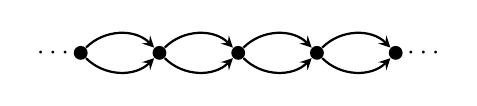
\begin{tikzpicture}[>=stealth]

\node [fill=black,black,circle,inner sep=0pt,minimum size=.5em] at (0,0) (s0) {};
\node [fill=black,black,circle,inner sep=0pt,minimum size=.5em] at (1,0) (s1) {};
\node [fill=black,black,circle,inner sep=0pt,minimum size=.5em] at (2,0) (s2) {};
\node [fill=black,black,circle,inner sep=0pt,minimum size=.5em] at (3,0) (s3) {};
\node [fill=black,black,circle,inner sep=0pt,minimum size=.5em] at (4,0) (s4) {};

\draw [->,thick] (s0) to [bend left=45] (s1);
\draw [->,thick] (s1) to [bend left=45] (s2);
\draw [->,thick] (s2) to [bend left=45] (s3);
\draw [->,thick] (s3) to [bend left=45] (s4);

\draw [->,thick] (s0) to [bend right=45] (s1);
\draw [->,thick] (s1) to [bend right=45] (s2);
\draw [->,thick] (s2) to [bend right=45] (s3);
\draw [->,thick] (s3) to [bend right=45] (s4);

\node (q0) [left of= s0,node distance=1em] {$\cdots$};
\node (q0) [right of= s4,node distance=1em] {$\cdots$};

\end{tikzpicture}

\end{document}
